\documentclass[conference]{IEEEtran}
\IEEEoverridecommandlockouts
% The preceding line is only needed to identify funding in the first footnote. If that is unneeded, please comment it out.
\usepackage{cite}
\usepackage{amsmath,amssymb,amsfonts}
\usepackage{algorithmic}
\usepackage{graphicx}
\usepackage{textcomp}
\usepackage{xcolor}
\usepackage{svg}
\usepackage{listings}
\usepackage{booktabs}
\usepackage[margin=1in]{geometry}
\usepackage{tabularx}
\usepackage{booktabs}
\usepackage{caption}
\usepackage[colorlinks=true, linkcolor=blue, urlcolor=blue]{hyperref}

\def\BibTeX{{\rm B\kern-.05em{\sc i\kern-.025em b}\kern-.08em
    T\kern-.1667em\lower.7ex\hbox{E}\kern-.125emX}}
\begin{document}

\title{MMI713 Term Project - Phase 3 Report\\
% {\footnotesize \textsuperscript{*}Note: Sub-titles are not captured in Xplore and
% should not be used}
%\thanks{Identify applicable funding agency here. If none, delete this.}
}

\author{\IEEEauthorblockN{Abdullah Emir Göğüsdere}
\IEEEauthorblockA{\textit{Electrical and Electronics Engineering} \\
\textit{Middle East Technical University}\\
Ankara, Turkey \\
e244307@metu.edu.tr}
%\and
%\IEEEauthorblockN{2\textsuperscript{nd} Given Name Surname}
%\IEEEauthorblockA{\textit{dept. name of organization (of Aff.)} \\
%\textit{name of organization (of Aff.)}\\
%City, Country \\
%email address or ORCID}
%\and
%\IEEEauthorblockN{3\textsuperscript{rd} Given Name Surname}
%\IEEEauthorblockA{\textit{dept. name of organization (of Aff.)} \\
%\textit{name of organization (of Aff.)}\\
%City, Country \\
%email address or ORCID}
%\and
%\IEEEauthorblockN{4\textsuperscript{th} Given Name Surname}
%\IEEEauthorblockA{\textit{dept. name of organization (of Aff.)} \\
%\textit{name of organization (of Aff.)}\\
%City, Country \\
%email address or ORCID}
%\and
%\IEEEauthorblockN{5\textsuperscript{th} Given Name Surname}
%\IEEEauthorblockA{\textit{dept. name of organization (of Aff.)} \\
%\textit{name of organization (of Aff.)}\\
%City, Country \\
%email address or ORCID}
%\and
%\IEEEauthorblockN{6\textsuperscript{th} Given Name Surname}
%\IEEEauthorblockA{\textit{dept. name of organization (of Aff.)} \\
%\textit{name of organization (of Aff.)}\\
%City, Country \\
%email address or ORCID}
}

\maketitle

\begin{abstract}
Solving large sparse linear systems efficiently is a fundamental challenge in scientific computing, particularly in fields like circuit simulation, structural analysis, and machine learning. The Conjugate Gradient (CG) algorithm is widely used for such problems, but its performance can be limited by sequential bottlenecks and memory-bound operations on traditional CPUs. This project presents a GPU-accelerated implementation of the CG method using CUDA, featuring a row binning strategy that assigns sparse and dense rows to separate CUDA kernels (spmv\_bin0\_kernel and spmv\_bin1\_kernel) for optimized execution. By using concurrent kernel launches via CUDA streams and carefully balancing workloads, the implementation achieves up to 39× speedup over a sequential CPU version on large benchmark matrices. The implementation code, data files (in .txt format), and documentation are available at: \href{https://github.com/yerminal/MMI713-Project}{GitHub Repository}.
\end{abstract}

\begin{IEEEkeywords}
Conjugate Gradient, Sparse Linear Systems, GPU Acceleration, CUDA, Sparse Matrix-Vector Multiplication, Stream Concurrency, Row Binning, Parallel Computing
\end{IEEEkeywords}

\section{Motivation \& Significance}
Solving large sparse linear systems efficiently is a fundamental challenge in many scientific and engineering applications. As system sizes and problem complexities increase in scientific and engineering computations, the time spent in communication and data exchange across processors can dominate the total computation time. This makes it inefficient to solve large-scale linear systems. For these systems, the Conjugate Gradient (CG) algorithm is one of the most widely used iterative solvers due to its low memory requirements and strong convergence properties \cite{b1}.

However, the performance of CG is heavily dependent on the efficiency of underlying linear algebra operations, particularly sparse matrix-vector multiplication (SpMV) and inner product calculations. With the increasing size and complexity of modern simulations, traditional CPU-based implementations often become a performance bottleneck. Usage of GPU acceleration provides an opportunity to significantly reduce solution time through parallelism \cite{b1}.

This work focuses on designing and implementing parallelized CG algorithm optimized for sparse matrices in compressed sparse row (CSR) format on NVIDIA GPUs. It uses strategies such as row binning, warp-level parallelism, and concurrent kernel execution to improve scalability and throughput. The ability to solve large-scale systems faster and more efficiently is crucial in enabling real-time simulation and faster iterative design in critical domains.

This report includes material from my earlier CENG577 coursework. Some parts are reused directly and all reused content is clearly cited to ensure academic honesty.

\section{Problem Statement}

\subsection{Conjugate Gradient (CG) Algorithm}

The CG algorithm is commonly used to find the minimum value of a multi-dimensional function. In the context of solving matrix equations, it solves the equation \(Ax = b\) to find \(x\), where \(A\) is a symmetric and positive-definite matrix, and b is the right-hand side vector. Here, the goal is to minimize the residual \( r = b - Ax \) \cite{b1}.

During each iteration, the estimated \(x\) solution is updated by moving a specific step size $\alpha$ along the search direction vector \(p\). The step size $\alpha$ is computed based on the current values of \(A\) and \(p\) at that iteration. The search direction \(p\) is adjusted based on changes in the norm of the residual, which also serves as a criterion for convergence.

The pseudo-code for sequential CG is provided below \cite{b1}:
{\tiny
\begin{align*}
p &= b \\
r &= b - Ax \\
&r_{\text{old}} = r \\
x &= x_0 \\
\text{\textbf{for} } i = &0 \text{ to maxIter do} \\
\alpha &= \frac{r \cdot r}{p \cdot Ap} \\
x &= x + \alpha p \\
r &= r - \alpha Ap \\
\text{\textbf{if} } &\sqrt{r \cdot r} < \text{tolerance then} \\
&\text{\quad\textbf{break}}  \\
\beta &= \frac{r \cdot r}{r_{\text{old}} \cdot r_{\text{old}}} \\
p &= r + \beta p \\
&r_{\text{old}} = r \\
\text{\textbf{Solution} } & \text{\textbf{is} } x
\end{align*}
}

\section{Prior Work \& Limitations}
Several strategies have been developed to address the challenge of efficient parallel implementation of the CG method. These approaches can be roughly categorized into pipelined CG methods and s-step (communication-avoiding) CG methods.

\subsection{Pipelined Conjugate Gradient methods}
These methods reduce the effect of global communication in CG by overlapping all-reduce operations, used for dot products, with independent computations like sparse matrix-vector multiplication (SPMV) and preconditioner application. This is accomplished using non-blocking communication primitives that allow the program to start the communication early in the iteration and continue with other tasks that don't depend on its result. As a result, communication latency is hidden behind ongoing computation which is minimizing the idle time of the processor and improving overall throughput \cite{b2}.

Research has extended the basic pipelined CG method to include "deeper pipelines" (p(l)-CG) \cite{b3}, where the global all-to-all reduction phase in each CG iteration is overlapped with not just one, but $l$ subsequent SPMV operations. This deeper pipelining is particularly advantageous when the global communication phase becomes the dominant factor limiting scalability, allowing for further performance improvements on systems with many processors. However, pipelining can impact numerical stability due to the reordering of computations and accumulation of rounding errors, potentially increasing the number of iterations required for convergence.

\subsection{s-step Conjugate Gradient methods}
s-step CG methods adopt a different strategy by reformulating the CG algorithm to perform a block of s iterations with significantly fewer global communication steps compared to the standard CG algorithm. This reduction in communication is typically achieved by generating a basis for an s-dimensional Krylov subspace within each block of iterations using mostly local operations. By performing multiple SPMVs and other local computations within each s-step block before any global communication occurs, the communication cost is reduced over s iterations, effectively lowering the communication overhead per iteration \cite{b4}. 

A significant challenge associated with this method is maintaining numerical stability. The repeated SPMV operations within each block can lead to the generation of ill-conditioned Krylov bases resulting in potentially causing a loss of accuracy or slower convergence in finite precision arithmetic.

\section{Theory / Algorithm}
I propose a parallelized Conjugate Gradient (CG) solver which uses CUDA-based GPU acceleration to efficiently solve large sparse linear systems. This approach aims to improve performance by maximizing memory throughput and exploiting warp-level parallelism.

The block diagram in Fig.~\ref{figflow} illustrates the overall workflow of the proposed solver. 

\begin{figure}[htbp]
\centerline{\includesvg[width=\linewidth]{Picture1.svg}}
\caption{The block diagram of the overall workflow of proposed solver.}
\label{figflow}
\end{figure}

The process begins with reading the sparse matrix $A$ (in CSR format) and right-hand-side vector $b$ on the CPU. During preprocessing, the rows of the matrix are analyzed and divided into two bins based on row density (Bin0 for sparse rows, Bin1 for denser rows). 

All necessary data, including matrix arrays, vectors, and bin indices, are then transferred to the GPU. The parallelized CG algorithm executes iteratively on the GPU where sparse matrix-vector multiplications are computed using two kernels in separate CUDA streams to maximize parallelism. 

Each iteration includes vector updates, dot products, and convergence checks. Once the solution vector $x$ is computed, it is transferred back to the CPU for verification by comparing $Ax$ with $b$. The result is evaluated for accuracy and correctness.

\subsection{Parallelized CG Algorithm}
The CG algorithm is inherently well-suited for data-based parallelism, where data and associated operations are distributed among processing units. In contrast, task-based parallelism, where each processor handles a distinct task, is less applicable here. This is evident from the pseudo-code of sequential CG, where most steps rely on the results of previous steps, leaving limited scope for task-based parallelism \cite{b1}.

The pseudo-code for the parallelized CG algorithm is provided below:
{\tiny
\begin{align*}
p^{\text{device}} &= b^{\text{device}} \\
r^{\text{device}} &= b^{\text{device}} \\
\text{dot}_{\text{r}_{\text{old}}}^{\text{device}} &= r^{\text{device}} \cdot r^{\text{device}} \\
\text{dot}_{\text{r}_{\text{old}}}^{\text{host}} &= \text{dot}_{\text{r}_{\text{old}}}^{\text{device}} \\
x^{\text{device}} &= 0 \\
\text{\textbf{for} } i = 0 \text{ to } \text{max} & \text{Iter \textbf{do}} \\
(Ap)^{\text{device}} &= \text{SpMV}(A^{\text{device}},\, p^{\text{device}}) \\
\text{dot}_{\text{pAp}}^{\text{device}} &= p^{\text{device}} \cdot (Ap)^{\text{device}} \\
\text{dot}_{\text{pAp}}^{\text{host}} &= \text{dot}_{\text{pAp}}^{\text{device}} \\
\alpha^{\text{host}} &= \frac{\text{dot}_{\text{r}_{\text{old}}}^{\text{host}}}{\text{dot}_{\text{pAp}}^{\text{host}}} \\
x^{\text{device}} &= x^{\text{device}} + \alpha^{\text{host}} p^{\text{device}} \\
r^{\text{device}} &= r^{\text{device}} - \alpha^{\text{host}} (Ap)^{\text{device}} \\
\text{dot}_{\text{r}}^{\text{device}} &= r^{\text{device}} \cdot r^{\text{device}} \\
\text{dot}_{\text{r}}^{\text{host}} &= \text{dot}_{\text{r}}^{\text{device}} \\
\text{\textbf{if} } \sqrt{\text{dot}_{\text{r}}^{\text{host}}} &< \text{tolerance \textbf{then}} \\
\quad \text{\textbf{break}} & \\
\beta^{\text{host}} &= \frac{\text{dot}_{\text{r}}^{\text{host}}}{\text{dot}_{\text{r}_{\text{old}}}^{\text{host}}} \\
\text{dot}_{\text{r}_{\text{old}}}^{\text{host}} &= \text{dot}_{\text{r}}^{\text{host}} \\
p^{\text{device}} &= r^{\text{device}} + \beta^{\text{host}} p^{\text{device}} \\
x^{\text{host}} &= x^{\text{device}} \\
\text{\textbf{Solution is} } x^{\text{host}} &
\end{align*}
}

Where:

\begin{itemize}
\item the matrix and vector portions residing in GPU memory are denoted by device, in CPU memory are denoted by host.
\item $\cdot$ in $r^{\text{device}} \cdot r^{\text{device}}$ represents the dot product,
\item $\text{dot}_{\text{r}}$ represents the dot product of r,
\item SpMV represents the sparse matrix-vector multiplication.
\end{itemize}

\subsection{Matrix storage format}

Sparse matrices, where many of their elements are zero, commonly appear in scientific computing. We can use the sparse nature of these matrices to improve performance by storing and working with only the non-zero elements. A simple method for this is called Compressed Sparse Row (CSR) format \cite{b1}.

CSR is crucial for efficiently storing and processing sparse matrices. It reduces memory usage by storing only non-zero elements and their positions, making it ideal for large, sparse matrices. CSR is especially efficient for operations like sparse matrix-vector multiplication and is widely used in scientific computing due to its compatibility with parallel processing and numerical libraries \cite{b1}.

CSR represents a matrix using three arrays:
\begin{itemize}
\item \textbf{Values}: Non-zero elements row-wise.
\item \textbf{Column Indices}: Column positions of the non-zero elements.
\item \textbf{Row Pointers}: Start and end of each row in Values array.
\end{itemize}
Due to these advantages, all matrices in the implementation are stored in CSR format.

\subsection{Parallelization}
In the implementation, parallelization of CG operations is achieved primarily through CUDA-based kernel execution.

\subsubsection{SpMV - sparse matrix-vector multiplication}
The most computationally intensive operation, sparse matrix-vector multiplication (SpMV), is optimized by separating matrix rows based on total number of nonzero in a row to enable load balancing. The management of this separation is handled by a method called row binning.

Row binning analyzes the number of nonzero elements in each row of the sparse matrix during the preprocessing stage on the CPU. For each row, the number of nonzeros is calculated by subtracting consecutive entries in the CSR row\_ptr array. Based on a predefined threshold (e.g., 16 nonzeros), rows are categorized into two groups: low-density and high-density. 

The indices of low-density rows are stored in a separate array (bin0\_rows), while the indices of high-density rows are stored in another array (bin1\_rows). These arrays are then transferred to GPU memory.

SpMV operation is divided into two specialized kernels: one is “spmv\_bin0\_kernel” and the other is “spmv\_bin1\_kernel”. During SpMV execution on the GPU, spmv\_bin0\_kernel uses bin0\_rows to launch one thread per row for low-density rows, and spmv\_bin1\_kernel uses bin1\_rows to launch one warp per row for high-density rows.

For spmv\_bin0\_kernel, rows with relatively few nonzeros (e.g., 16 or fewer) are assigned to spmv\_bin0\_kernel, where each row is processed by a single thread—this is efficient because the workload is small and thread-level parallelism suffices. The pseudo code for spmv\_bin0\_kernel is given below:

\lstset{
  basicstyle=\ttfamily\tiny,
  keywordstyle=\color{blue}\bfseries,
  identifierstyle=\color{black},
  commentstyle=\color{gray},
  stringstyle=\color{red},
  showstringspaces=false,
  breaklines=true
}

\begin{lstlisting}[language=C]
kernel spmv\_bin0\_kernel(row_ids, num_rows, row_ptr, col_ind, val, x, y):
    thread_id = blockIdx.x * blockDim.x + threadIdx.x

    if thread_id >= num_rows:
        return

    row = row_ids[thread_id]
    sum = 0

    for j from row_ptr[row] to row_ptr[row + 1] - 1:
        sum += val[j] * x[col_ind[j]]

    y[row] = sum
\end{lstlisting}

In contrast, rows with more nonzeros are assigned to spmv\_bin1\_kernel, where each row is handled by an entire warp (32 threads) benefiting the warp-level parallelism to compute partial sums in parallel. Then, partial sums are reduced efficiently using warp shuffle operations that do not require the use of shared memory.

The pseudo code for spmv\_bin1\_kernel is given below:
\begin{lstlisting}[language=C]
kernel spmv\_bin1\_kernel(row_ids, num_rows, row_ptr, col_ind, val, x, y):
  global_warp_id = (blockIdx.x * blockDim.x + threadIdx.x) / WARP_SIZE
  lane = threadIdx.x % WARP_SIZE

  if global_warp_id >= num_rows:
    return

  row = row_ids[global_warp_id]
  sum = 0

  // Each thread in the warp processes a subset of the row
  for j from row_ptr[row] + lane to row_ptr[row + 1] - 1 step WARP_SIZE:
    sum += val[j] * x[col_ind[j]]

  // Perform warp-wide reduction using shuffle instructions
  for offset = WARP_SIZE / 2 down to 1 step /= 2:
    sum += warp_shfl_down(sum, offset)

  if lane == 0:
    y[row] = sum
\end{lstlisting}

Lastly, these two kernels are launched in separate CUDA streams to allow concurrent execution when hardware resources are sufficient. This selective kernel strategy makes sure better load balancing and efficient utilization of GPU threads across a wide range of sparse matrix structures.

\subsection{Vector updates and dot products}
Other CG operations such as vector updates and dot products are also parallelized across threads using standard 1D grid-block configurations. This approach ensures that all stages of the CG iteration can exploit the high parallelism offered by the GPU architecture. Additionally, dot product kernel uses shared memory and atomicAdd for safe accumulation across blocks.
The pseudo code for dot product kernel is given below:
\begin{lstlisting}[language=C]
kernel vector_dot(a, b, result, n):
  shared temp[blockDim.x]
  tid = threadIdx.x
  i = blockIdx.x * blockDim.x + tid

  if i < n:
    temp[tid] = a[i] * b[i]
  else:
    temp[tid] = 0

  __syncthreads()
  // Parallel reduction in shared memory
  for offset = blockDim.x / 2 down to 1 step /= 2:
    if tid < offset:
      temp[tid] += temp[tid + offset]
    __syncthreads()

  if tid == 0:
    atomicAdd(result, temp[0])
\end{lstlisting}

\subsection{Memory Usage}
Memory usage in this implementation is designed to use the GPU’s memory efficiently. All vectors and matrix data (in CSR format) are allocated in global memory, while shared memory is used in the dot product kernel to enable fast intra-block reductions. 

Intermediate scalars used in convergence checks and coefficient calculations are kept in device memory and are accessed via cudaMemcpy only when necessary. Careful synchronization and memory allocation strategies help avoid race conditions and minimize latency.

\section{Experiments or other Evidence of Success}

\subsection{Parameter Settings}
The following parameter settings were used to optimize performance and ensure correct convergence:
\begin{itemize}
\item \textbf{Maximum Iterations (MAX\_ITERS)}: Set to 10,000 to ensure sufficient opportunity for convergence, particularly for ill-conditioned matrices.
\item \textbf{Tolerance (TOL)}: A convergence threshold of 1e-11 was used, terminating iterations when the residual norm falls below this value.
\item \textbf{Thread Block Configuration}: For vector operations and spmv\_bin0\_kernel, a fixed block size of 256 threads was used. This setting was chosen based on typical occupancy and warp scheduling considerations on modern GPUs.
\item \textbf{Warp-Based SpMV Configuration}: For spmv\_bin1\_kernel, 32-thread warps were grouped into blocks of 4 warps (i.e., THREADS\_BIN1 = 128) to ensure balanced workload distribution and efficient warp utilization.
\item \textbf{Binning Threshold}: Rows with 16 or fewer nonzeros were assigned to Bin0, while rows with more than 16 nonzeros were assigned to Bin1.
\item \textbf{CUDA Streams}: Two streams were used to enable concurrent execution of spmv\_bin0\_kernel and spmv\_bin1\_kernel, improving throughput by overlapping execution when hardware resources allow.
\end{itemize}

\subsection{Dataset}
Sparse matrices used in this experiment were sourced from the Suite Sparse Matrix Collection \cite{b5} and represented in the Compressed Sparse Row (CSR) format due to its memory efficiency and suitability for SpMV operations. Additionally, a custom symmetric positive definite (SPD) matrix was generated in MATLAB to test balanced binning scenarios.

The dataset files, containing both the problem matrix and the right-hand side vector, were stored in .txt format for simplicity and ease of integration. The implementation reads four separate files: one for the Row Pointers, one for the Column Indices, one for the Values of the matrix, and one for the values of the right-hand side vector b.

\subsection{Experimental Procedure}
Two algorithmic approaches were used in the experiments: a CPU-based sequential Conjugate Gradient (CG) algorithm and a GPU-accelerated parallel CG implementation using CUDA. Both methods solve the same set of sparse linear systems using identical matrix and vector inputs to ensure fair comparison.

For each matrix, the total execution time of the CG solver was recorded. In the GPU implementation, CUDA event timers were used to measure kernel-level timings, including the combined time of spmv\_bin0\_kernel and spmv\_bin1\_kernel, as well as their individual execution times. The CPU execution time was recorded using wall-clock timing in C++.

To evaluate performance, speedup was computed as the ratio of CPU time to GPU time. Additionally, other metrics such as the number of CG iterations to converge and the row binning distribution (size of bin0 and bin1) were collected for each matrix. This procedure was repeated for all datasets, including standard benchmarks and the custom SPD matrix. The resulting data was then analyzed to understand the effect of matrix structure, kernel concurrency, and binning balance on performance.


\subsection{Results}
Tables~\ref{tableSpeed} and~\ref{tableTime} present the results of performance experiments comparing CPU and GPU implementations of the Conjugate Gradient (CG) algorithm on a range of sparse matrices. Table~\ref{tableDataset} provides structural information about each matrix, including the number of rows, columns, and nonzero entries, as well as the condition number where available. The condition number provides an indication of the expected convergence rate in the CG method—larger condition numbers generally lead to slower convergence and require more iterations. The right-hand side (RHS) vectors for all test cases were randomly generated in MATLAB to simulate general-purpose input. Table~\ref{tableDataset} also includes size(Bin0) and size(Bin1), which represent the number of rows assigned to two specialized SpMV kernels based on row sparsity—Bin0 for rows with fewer nonzeros (handled using a thread-per-row strategy), and Bin1 for denser rows (processed with a warp-per-row strategy). For entries marked N/A, the condition number was not specified or not available.

Table~\ref{tableTime} summarizes the performance results, including the number of CG iterations until convergence, the total CPU execution time, and three GPU timing metrics. GPU Time 1 reports the total execution time when both SpMV kernels are launched concurrently in separate CUDA streams. GPU Time 2 and GPU Time 3 show the individual execution times of spmv\_bin0\_kernel and spmv\_bin1\_kernel, respectively, when measured in isolation. These results help assess the performance benefits of GPU acceleration, the effectiveness of the binning strategy, and the impact of concurrency on execution time across different matrix types.

\begin{table}[htbp]
\centering
\tiny
\caption{Structural Information Table for Sparse Matrices}
\begin{tabular}{lrrrrrrrrrrr}
\hline
Matrix & Rows & Columns & Nonzeros & Cond. Num. & size(Bin0) & size(Bin1) \\
\hline
\href{https://sparse.tamu.edu/HB/bcsstm09}{HB/bcsstm09}    & 1083   & 1083   & 1,083     & 1.00E+04   & 1083   & 0     \\
\href{https://sparse.tamu.edu/HB/nos3}{HB/nos3}        & 960    & 960    & 15,844    & 3.77E+04   & 245    & 715    \\
\href{https://sparse.tamu.edu/HB/bcsstk27}{HB/bcsstk27}    & 1224   & 1224   & 56,126    & 2.41E+04   & 4      & 1224    \\
\href{https://sparse.tamu.edu/Pothen/bodyy5}{Pothen/bodyy5}  & 18589  & 18589  & 128,853   & 7.87E+03   & 18589  & 0       \\
\href{https://sparse.tamu.edu/MathWorks/Kuu}{MathWorks/Kuu}  & 7102   & 7102   & 340,200   & 1.58E+04   & 0      & 7102    \\
\href{https://sparse.tamu.edu/UTEP/Dubcova2}{UTEP/Dubcova2}  & 65025  & 65025  & 1,030,225 & N/A        & 48900  & 16125  \\
Custom SPD  & 30000  & 30000  & 4,543,292 & N/A        & 14950  & 15050  \\
\hline
\end{tabular}
\label{tableDataset}
\end{table}

\begin{table}[htbp]
\centering
\tiny
\caption{Speedup Table for Sparse Matrices}
\begin{tabular}{lrrrrrr}
\hline
Matrix & CPU Time & GPU Time 1 & Speedup (CPU/GPU1) \\
\hline
\href{https://sparse.tamu.edu/HB/bcsstm09}{HB/bcsstm09}     & \textbf{0.2864 ms}   & 1.576 ms  & 0.18$\times$ \\
\href{https://sparse.tamu.edu/HB/nos3}{HB/nos3}        		  & \textbf{47.0606 ms}  & 88.385 ms  & 0.53$\times$ \\
\href{https://sparse.tamu.edu/HB/bcsstk27}{HB/bcsstk27}      & 514.721 ms           & \textbf{349.772 ms} & 1.47$\times$ \\
\href{https://sparse.tamu.edu/Pothen/bodyy5}{Pothen/bodyy5}  & 1392.49 ms           & \textbf{208.902 ms} & 6.66$\times$ \\
\href{https://sparse.tamu.edu/MathWorks/Kuu}{MathWorks/Kuu}  & 1702.81 ms           & \textbf{212.625 ms} & 8.01$\times$ \\
\href{https://sparse.tamu.edu/UTEP/Dubcova2}{UTEP/Dubcova2}  & 3484.62 ms           & \textbf{94.571 ms}  & 36.85$\times$ \\
Custom SPD     															& 612.47 ms            & \textbf{15.6725 ms} & 39.07$\times$ \\
\hline
\end{tabular}
\label{tableSpeed}
\end{table}

\begin{table}[htbp]
\centering
\tiny
\caption{Comparison of CPU and GPU Execution Times for Sparse Matrices}
\begin{tabular}{lrrrrrrrrrrr}
\hline
Matrix & Iteration & CPU Time & GPU Time 1 & GPU Time 2 & GPU Time 3  \\
\hline
\href{https://sparse.tamu.edu/HB/bcsstm09}{HB/bcsstm09}      & 4    & \textbf{0.2864 ms}   & 1.576 ms   & 1.437 ms   & 2.427 ms \\
\href{https://sparse.tamu.edu/HB/nos3}{HB/nos3}        		   & 512  & \textbf{47.0606 ms}  & 88.385 ms  & 101.563 ms & 93.077 ms \\
\href{https://sparse.tamu.edu/HB/bcsstk27}{HB/bcsstk27}       & 2201 & 514.721 ms  & \textbf{349.772 ms} & 432.524 ms & 352.226 ms \\
\href{https://sparse.tamu.edu/Pothen/bodyy5}{Pothen/bodyy5}  & 1315 & 1392.49 ms  & \textbf{208.902 ms} & 210.487 ms & 287.084 ms \\
\href{https://sparse.tamu.edu/MathWorks/Kuu}{MathWorks/Kuu}  & 1151 & 1702.81 ms  & 212.625 ms & 270.940 ms & \textbf{210.663 ms} \\
\href{https://sparse.tamu.edu/UTEP/Dubcova2}{UTEP/Dubcova2}   & 506  & 3484.62 ms  & 94.571 ms  & \textbf{90.035 ms}  & 154.422 ms \\
Custom SPD  																& 38  & 612.47 ms  & \textbf{15.6725 ms} & 268.503 ms & 18.1784 ms  \\
\hline
\end{tabular}
\label{tableTime}
\end{table}

In Table~\ref{tableTime}, the results demonstrate the effectiveness and scalability of our GPU-accelerated Conjugate Gradient (CG) method across a diverse set of sparse matrices. For small matrices such as HB/bcsstm09 and HB/nos3, the GPU implementation yields limited benefit due to the low computational intensity which is shown by the smaller execution time on the CPU than the one on the GPU. However, for larger and more complex matrices such as HB/bcsstk27, MathWorks/Kuu, and UTEP/Dubcova2 the GPU significantly outperforms the CPU. For example, in Dubcova2, it completes in 94.571 ms on the GPU versus 3484.62 ms on the CPU resulting in a speedup of 36.85$\times$, even with over 2200 CG iterations. This gain is largely credited to efficient handling of dense rows via the warp-based spmv\_bin1\_kernel.

For bcsstk27, bodyy5, and Kuu, the GPU Time 1 closely matches the execution time of the dominant SpMV kernel. This is because the row binning is highly unbalanced in these matrices, nearly all rows fall into either bin0 or bin1. As a result, only one type of kernel is predominantly launched and the contribution of the other kernel is minimal. This skewed bin distribution leads to minimal overlap between the two kernels which is making the GPU Time 1 effectively determined by the heavier bin's execution.

In the case of Dubcova2, although it is the largest matrix in the dataset, with over 65,000 rows and more than one million nonzeros, it achieves excellent GPU performance due to the binning structure and the low iteration count. Approximately 75\% of the rows (48,900) fall into bin0, each having 16 or fewer nonzeros, and are processed by spmv\_bin0\_kernel using a thread-per-row strategy. The remaining 25\% (16,125 rows) fall into bin1 where every one of these rows are processed by spmv\_bin0\_kernel using a warp-per-row strategy. Another reason for the exceptional performance in Dubcova2 is that it converges in just 506 iterations which are much fewer than those in matrices like bcsstk27 (which takes 2201 iterations) or nos3 (512 iterations). Since matrix-vector multiplications dominate the cost per iteration in CG, a low iteration count directly translates into faster overall convergence and lower runtime. The combined execution of spmv\_bin0\_kernel and spmv\_bin1\_kernel, launched in separate CUDA streams, results in a total GPU time of 94.57 ms despite the individual kernel times being 90.03 ms and 154.42 ms respectively. This shows a stream-level concurrency where the kernels partially overlap in execution which is reducing the runtime. This stream-level concurrency between spmv\_bin0\_kernel and spmv\_bin1\_kernel is illustrated in Fig.~\ref{timelineFig} and Fig.~\ref{eventsFig} which are captured from the trace output of Nsight Systems 2025.1.3.
 
\begin{figure}[htbp]
\centering
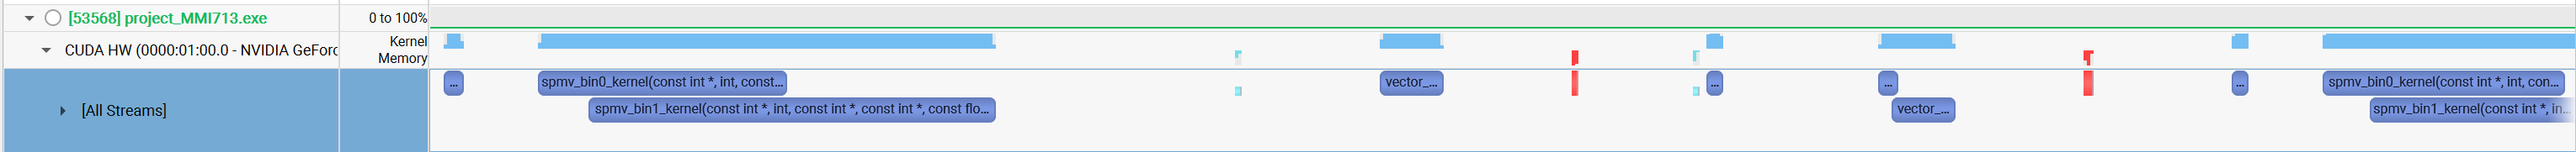
\includegraphics[width=\columnwidth]{timeline.png}
\caption{Cropped timeline view of the GPU implementation.}
\label{timelineFig}
\end{figure}

\begin{figure}[htbp]
\centering
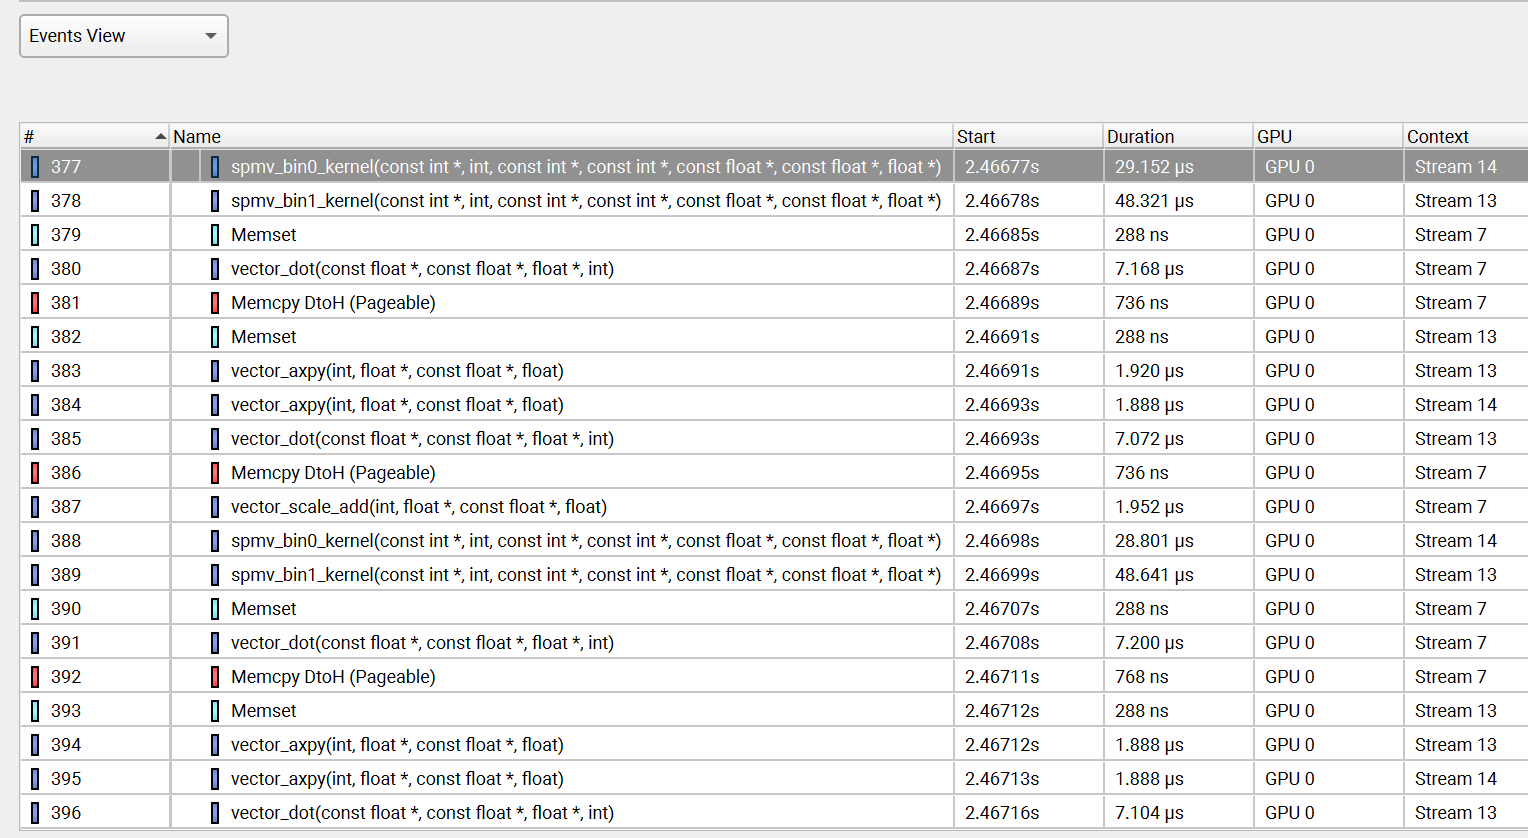
\includegraphics[width=\columnwidth]{events.png}
\caption{Cropped event view of the GPU implementation.}
\label{eventsFig}
\end{figure}

In Table~\ref{tableTime}, it is observed that spmv\_bin0\_kernel alone appears faster than the combined execution of spmv\_bin0\_kernel + spmv\_bin1\_kernel in Dubcova2. The reason is that when measuring spmv\_bin0\_kernel in isolation, it runs without any other kernel occupying GPU resources. This allows it to use more of the GPU's compute and memory bandwidth. But when both kernels are launched together in separate streams, they compete for shared resources which may slightly delay the execution of bin0 internally even though the total time (combined) becomes shorter due to overlap. Another reason is that in bin1, each row contains exactly 25 nonzeros, which results in underutilization of GPU warps. Since each warp consists of 32 threads but only 25 elements need to be processed per row, the remaining 7 threads in each warp remain idle which is reducing the overall efficiency. In contrast, bin0 uses a thread-per-row strategy, which is better suited for the irregular but small row sizes in that bin and achieves higher utilization. In the case of nos3 where the rows of its bin1 have at least 32 nonzeros, the combined execution of spmv\_bin0\_kernel and spmv\_bin1\_kernel is actually faster than running each kernel alone. This indicates that the GPU has sufficient resources such as shared memory, execution units, and memory bandwidth to accommodate both kernels concurrently without introducing significant delays. As a result, both kernels can execute efficiently in parallel while benefiting from overlap without degrading each other’s performance.

To evaluate performance under balanced binning conditions, a custom symmetric positive definite (SPD) matrix was generated in MATLAB, where rows in bin0 each contain 10 nonzeros and rows in bin1 contain 64 nonzeros. The matrix was designed with nearly equal bin sizes and appropriate row density (14,950 rows with 10 nonzeros in bin0 and 15,050 rows with 64 nonzeros in bin1) to ensure a well-balanced workload between the two SpMV kernels. Due to this balance, both spmv\_bin0\_kernel and spmv\_bin1\_kernel are actively utilized and executed concurrently in separate CUDA streams. As a result, for Custom SPD in Table~\ref{tableTime}, the total GPU execution time (GPU Time 1) is shorter than either kernel’s individual runtime, clearly demonstrating the benefits of balanced row distribution and effective kernel overlap.

In conclusion, the results show that the GPU-based Conjugate Gradient (CG) method performs best when the matrix structure and workload distribution are well balanced. While small matrices don’t gain much speedup due to low computation per iteration, larger matrices with many nonzeros and structured sparsity show significant improvements. Dividing matrix rows into two bins—one for rows with fewer nonzeros (handled by spmv\_bin0\_kernel) and one for denser rows (handled by spmv\_bin1\_kernel)—helps match the kernel strategy to the data pattern. When these two kernels are launched in separate CUDA streams, they can run at the same time, reducing overall execution time. However, this only works well if the GPU has enough resources and the row sizes are suited to the kernel. For example, in Dubcova2, rows in bin1 have exactly 25 nonzeros, which leads to underuse of GPU threads in a warp, slightly lowering performance. Still, thanks to a high percentage of simple rows in bin0 and a low number of CG iterations, Dubcova2 runs very efficiently on the GPU. A custom balanced matrix also confirms that when the workload between the two bins is even, both kernels can overlap effectively, resulting in better overall performance. This highlights the importance of load balancing and stream concurrency when optimizing CG on GPUs.


\section{Discussion and Future Work}
The results of this study highlight the effectiveness of stream-level concurrency and bin-based kernel decomposition in accelerating the Conjugate Gradient (CG) method on GPUs. By dividing matrix rows into two categories based on sparsity and assigning them to specialized kernels (spmv\_bin0\_kernel and spmv\_bin1\_kernel), the implementation achieves better load balancing and improved resource utilization. Launching these kernels in separate CUDA streams enables concurrent execution, which, when combined with a balanced bin distribution, leads to significant reductions in total execution time. This effect is particularly pronounced in matrices with a large number of rows and structured sparsity, such as Dubcova2 and the custom SPD matrix, where speedups exceeded 30× over CPU execution. 

However, several limitations are evident. The use of a fixed binning threshold does not generalize well across all matrices, and resource contention between concurrent kernels can sometimes reduce the efficiency of individual kernels, even if the total time improves. Additionally, the implementation lacks support for preconditioning, which is often essential for solving ill-conditioned systems efficiently. The design is also limited to single-GPU environments and does not address scalability across multiple GPUs or distributed systems. Despite these limitations, the proposed method is well-suited for large-scale, symmetric positive definite problems common in scientific simulations and engineering applications. 

Future work should focus on adaptive or multi-bin strategies for more flexible row classification, integration of GPU-friendly preconditioners, and extension to multi-GPU or hybrid CPU-GPU architectures. Further enhancements such as auto-tuning of kernel configurations and benchmarking against established libraries like cuSPARSE would also provide deeper insight into the competitiveness and generalizability of the proposed approach.



\begin{thebibliography}{00}
\bibitem{b1} A. E. Gogusdere, “CENG577 - Final Project Report,” METU, Ankara, 2025.
\bibitem{b2} P. Ghysels and W. Vanroose, “Hiding global synchronization latency in the preconditioned Conjugate Gradient algorithm,” Parallel Computing, vol. 40, no. 7, pp. 224–238, Jun. 2013, doi: 10.1016/j.parco.2013.06.001.
\bibitem{b3} J. Cornelis, S. Cools, and W. Vanroose, “The Communication-Hiding Conjugate Gradient Method with Deep Pipelines,” arXiv.org, Jan. 15, 2018. https://arxiv.org/abs/1801.04728
\bibitem{b4} A. T. Chronopoulos and C. W. Gear, “s-step iterative methods for symmetric linear systems,” Journal of Computational and Applied Mathematics, vol. 25, no. 2, pp. 153–168, Feb. 1989, doi: 10.1016/0377-0427(89)90045-9.
\bibitem{b5} “SuiteSparse Matrix Collection,” the University of Florida, [Online]. Available: https://sparse.tamu.edu/. [Accessed 2025].

\end{thebibliography}

\end{document}
